\documentclass[11pt,a4paper]{article}
\usepackage[hmargin=2cm, vmargin=1.5cm]{geometry}
\usepackage{amsmath,amssymb}
\usepackage{graphicx}
\usepackage{hyperref}

\newcommand{\E}{\mathbb{E}}
\newcommand{\norm}[1]{\left\| #1 \right\|}

\title{Optimal minibatch size of SGD-NICE}
\author{Gor Melkumyan}
\date{}

\begin{document}
\maketitle

\section*{Idea}

The idea is to find empirically the best minibatch size $\tau$ of SGD-NICE and to compare it with the theoretical
optimal minibatch size $\tau^\star$. We use the same linear regression on the California housing data as in
\texttt{hw\_2026\_11\_11/sgd\_lin.ipynb}, with $n = 16512$, so all the constants $\mu$, $L$, $\max_i L_i$ and
$\sigma_\star^2$ are known.

For $\tau$ from $1$ to $n$ we run SGD-NICE with the stepsize of the convergence theorem and count how many gradients
are computed until $\E\bigl[\norm{w^k - w^\star}^2\bigr] \le 2\delta\norm{w^0 - w^\star}^2$ with $\delta = 0.005$
(the expectation is estimated with $10$ runs). One iteration of SGD-NICE costs $\tau$ gradients, and one iteration
of GD costs $n$. The theoretical curve is $\tau\,k(\tau)$, where $k(\tau)$ is the number of iterations from the
theorem.

The code is the file
\href{https://github.com/Gor-2001/thesis_hw/blob/main/Homework/Exercises/hw_2026_11_20/optimal_batch_size.ipynb}{\texttt{Homework/Exercises/hw\_2026\_11\_20/optimal\_batch\_size.ipynb}}.

\section*{Result}

\begin{center}
  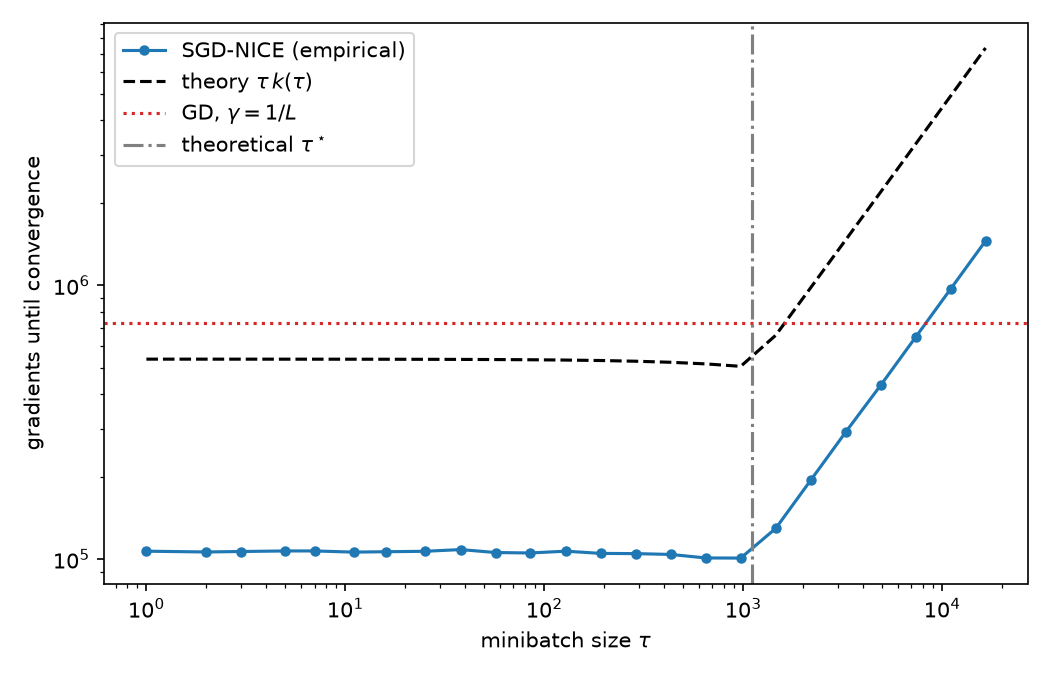
\includegraphics[width=0.75\textwidth]{figures/optimal_batch_size.png}
\end{center}

The theoretical optimal minibatch size is $\tau^\star \approx 1106$, and the empirical one is $\tau = 971$.
Up to $\tau^\star$ the number of gradients is almost constant (about $10^5$), and after it the number grows
linearly with $\tau$. The empirical curve has the same shape as the theoretical one and is about $5$ times below it.

\end{document}
